\documentclass[conference]{IEEEtran}

\usepackage[T1]{fontenc}
\usepackage{cite}
\usepackage{amsmath,amssymb,amsfonts}
\usepackage{algorithmic}
\usepackage{graphicx}
\usepackage{booktabs}
\usepackage{multirow}
\usepackage{array}
\usepackage{url}
\usepackage{tikz}
\usepackage{pgfplots}
\usepackage{siunitx}
\usepackage{enumitem}
\usepackage{xcolor}
\usepackage{threeparttable}
\usepackage{tabularx}
\usepackage{balance}

\pgfplotsset{compat=1.18}
\usetikzlibrary{arrows.meta, positioning, shapes.geometric, fit, calc}

\begin{document}

\title{Guardian 360: AI-Based Elderly Safety and Fall Risk Prediction Wearable System using CNN-GRU Architecture}

\author{
\IEEEauthorblockN{Author Name(s)}
\IEEEauthorblockA{
Department of Electronics and Communication Engineering\\
JSS Academy of Technical Education, Bengaluru, India\\
Email: author@institution.edu}
}

\maketitle

\begin{abstract}
The increasing elderly population and rising prevalence of mobility-related injuries necessitate intelligent, real-time, and proactive healthcare monitoring systems capable of detecting and predicting fall events before severe injury occurs. This paper presents \textit{Guardian 360}, an AI-based wearable elderly safety system designed for continuous gait analysis, fall risk prediction, real-time fall detection, and emergency alert generation using embedded edge intelligence. The proposed system integrates wearable inertial sensing, physiological monitoring, IoT connectivity, and a lightweight hybrid CNN-GRU deep learning architecture for predictive healthcare monitoring. The wearable platform combines an ESP32 microcontroller, MPU6050 inertial measurement unit, MAX30102 pulse oximeter, GPS module, OLED display, SOS trigger, and buzzer to perform multimodal health and movement monitoring in real time. A lightweight convolutional neural network (CNN) extracts local motion signatures from accelerometer and gyroscope streams, while a gated recurrent unit (GRU) captures temporal gait dependencies to classify normal gait, abnormal gait, fall risk, and fall events. Compared with traditional threshold-based and shallow machine learning systems, the proposed approach emphasizes predictive monitoring by identifying instability patterns before fall occurrence. Literature-guided analysis indicates that CNN-GRU provides an effective trade-off between classification accuracy, inference speed, memory efficiency, and embedded deployability. The system is designed for low-latency edge execution using TensorFlow Lite and Firebase-enabled caregiver monitoring, enabling real-time alerts and remote supervision. Guardian 360 demonstrates a practical and implementation-oriented framework for embedded AI in elderly care, contributing toward proactive, lightweight, and scalable predictive healthcare systems for assisted independent living.
\end{abstract}

\begin{IEEEkeywords}
Elderly healthcare, wearable IoT, fall risk prediction, gait analysis, CNN-GRU, embedded AI, TinyML, edge intelligence, predictive healthcare
\end{IEEEkeywords}

\section{Introduction}
The rapid growth of the aging population has increased the demand for intelligent healthcare systems capable of supporting safe and independent living among elderly individuals. Falls remain one of the most critical causes of injury, hospitalization, and mortality in older adults, often resulting in long-term disability and reduced quality of life. Conventional fall detection systems are primarily reactive, identifying a fall only after its occurrence. Such systems reduce response time but fail to prevent injuries caused by gait instability, imbalance, and gradual locomotion degradation.

Recent advances in wearable sensing, embedded systems, and edge artificial intelligence have enabled real-time health monitoring platforms that support continuous elderly supervision. However, existing solutions largely focus on reactive monitoring, threshold-based alerts, or computationally expensive cloud-centric analytics. These limitations hinder deployment in low-power wearable systems requiring low latency, real-time responsiveness, and predictive intelligence.

This paper presents \textit{Guardian 360}, a wearable AI-based elderly safety system for proactive fall prevention and continuous health monitoring. The proposed system integrates inertial gait analysis, physiological sensing, edge AI, and IoT-enabled caregiver communication into a lightweight wearable architecture. Its core contribution is a hybrid CNN-GRU model that performs real-time gait analysis and fall risk prediction using inertial motion sequences. Unlike conventional systems that detect only completed falls, Guardian 360 predicts fall risk by identifying abnormal gait progression and instability signatures before impact.

The proposed architecture is designed for embedded deployment using low-power hardware and TensorFlow Lite inference, making it suitable for continuous wearable operation. By combining real-time sensing, lightweight deep learning, and remote monitoring, Guardian 360 aims to improve elderly safety through predictive and proactive healthcare intervention.

\section{Literature Survey}
Recent literature demonstrates substantial progress in wearable elderly healthcare systems, remote monitoring, and AI-based fall analysis. However, most existing systems remain reactive, computationally heavy, or insufficiently validated for embedded predictive deployment.

Salma \textit{et al.} presented a scoping review of remote monitoring systems and reported improved hospitalization outcomes and quality of life, but emphasized limited long-term and context-independent validation in elderly care systems \cite{salma2025}. Bandara \textit{et al.} proposed a non-invasive sensor platform for elderly monitoring using IoT and cloud communication, demonstrating robust real-time sensing but lacking predictive analytics for proactive intervention \cite{bandara2020}. Setu \textit{et al.} introduced IoMT-based elderly monitoring architectures with efficient communication pipelines, yet predictive intelligence remained absent \cite{setu2025,setu2024}. Similar limitations were reported in NodeMCU-based elderly monitoring systems that offered real-time alerts but relied on threshold logic without predictive modeling \cite{augastiny2023}.

Deep learning has significantly improved fall detection performance. Saraubon \textit{et al.} demonstrated an IoT-based elderly care system using CNN for acoustic fall detection and decision trees for inertial classification, achieving promising results but lacking predictive fall analysis \cite{saraubon2018}. Gaud \textit{et al.} proposed a CNN-BiLSTM fall detection model achieving high accuracy on SisFall, though the model focused solely on post-fall classification rather than pre-fall risk prediction \cite{gaud2025}. Li \textit{et al.} and Zhang \textit{et al.} showed that deep learning models outperform conventional machine learning for fall detection, but noted higher computational complexity and reduced suitability for low-power edge systems \cite{li2024,zhang2025}.

Recent studies highlight gait as a strong digital biomarker for fall risk and cognitive decline. Lim \textit{et al.} used temporal gait features and LightGBM to predict fall risk with high accuracy, but the approach was video-dependent and unsuitable for wearable deployment \cite{lim2024}. Tsiakiri \textit{et al.} showed that wearable gait analysis enables early dementia and instability detection, though standardized real-time wearable systems remain limited \cite{tsiakiri2025}. Comprehensive reviews further emphasize the need for multimodal, predictive, and embedded systems capable of real-world deployment \cite{ishaq2026,patel2023}.

\subsection{Literature Survey Table}
\begin{table*}[!t]
\centering
\caption{Summary of Recent Literature on Elderly Monitoring and Fall Analysis (Synthesized from Literature Matrix)}
\label{tab:litreview}
\scriptsize
\begin{threeparttable}
\begin{tabularx}{\textwidth}{p{1.2cm}p{2.6cm}p{2.5cm}p{2.0cm}p{2.0cm}p{2.4cm}p{2.7cm}}
\toprule
Year & Author(s) & Methodology & Dataset & Metrics & Key Results & Limitation / Gap \\
\midrule
2025 & Salma \textit{et al.} & RMS scoping review & 18 studies & Hospitalization, QoL & Reduced hospitalization, cost-effective monitoring & No robust long-term predictive evidence \\
2020 & Bandara \textit{et al.} & IoT sensor platform & Real-time wearable/environmental & Reliability, loss rate & Reliable remote monitoring & No predictive analytics \\
2024 & Setu \textit{et al.} & IoT smart elderly care & IoT physiological streams & Accuracy, response time & Improved monitoring and alerts & No personalization or predictive AI \\
2023 & Augastiny \textit{et al.} & NodeMCU IoT monitoring & Multi-sensor IoT & Accuracy, alert latency & Real-time elderly monitoring & Threshold-based, no prediction \\
2018 & Saraubon \textit{et al.} & CNN + DT fall detection & UCI + controlled data & Accuracy, Recall & Accurate real-time fall detection & No predictive fall analysis \\
2024 & Lim \textit{et al.} & Gait ML (LightGBM) & MMU-FRiP + Mendeley & Accuracy & High fall-risk prediction accuracy & Vision-based, not wearable \\
2025 & Gaud \textit{et al.} & 1D CNN + BiLSTM & SisFall & Accuracy, inference time & High detection accuracy & Detects fall, does not predict risk \\
2025 & Tsiakiri \textit{et al.} & Wearable gait review & 126 studies & Trend analysis & Gait useful for early decline detection & Limited real-time standardization \\
2026 & Ishaq \textit{et al.} & Fall review (130 studies) & Secondary review & F1, Sensitivity & Predictive shift toward DL systems & Poor real-world validation \\
2025 & Zhang \textit{et al.} & CNN/LSTM fall AI & Public fall datasets & Precision, Recall & High controlled-environment accuracy & High compute, limited real-world data \\
\bottomrule
\end{tabularx}
\end{threeparttable}
\end{table*}

\section{Research Gap}
The literature reveals four major limitations in current elderly safety systems:

\begin{enumerate}[leftmargin=*,noitemsep]
\item Most systems are \textbf{reactive}, detecting falls only after impact rather than predicting instability before fall occurrence.
\item Existing wearable solutions rely heavily on \textbf{threshold logic or shallow machine learning}, limiting predictive robustness.
\item Deep learning systems such as CNN-LSTM provide strong performance but are often \textbf{too computationally expensive for low-power wearable deployment}.
\item Real-time systems frequently lack \textbf{integrated multimodal monitoring}, combining gait, vitals, alerts, and caregiver communication in a unified edge AI framework.
\end{enumerate}

Therefore, a lightweight, predictive, and embedded AI architecture is required for proactive elderly fall prevention.

\section{Problem Statement}
Existing elderly safety systems predominantly detect fall events after occurrence, leading to delayed intervention and limited injury prevention. Traditional threshold-based wearables lack contextual understanding of gait instability, while cloud-dependent and computationally intensive AI systems are unsuitable for low-power continuous wearable deployment. There is a need for a lightweight wearable system capable of real-time gait analysis, fall risk prediction, physiological monitoring, and emergency alert generation using embedded AI for proactive elderly safety.

\section{Proposed System}
Guardian 360 is a wearable edge AI system designed for continuous elderly safety monitoring. The system performs:
\begin{itemize}[leftmargin=*]
\item Real-time fall detection
\item Gait analysis and instability assessment
\item Fall risk prediction
\item Physiological health monitoring
\item SOS and emergency alerting
\item Remote caregiver notification
\end{itemize}

The device is designed as a wrist/hand wearable and integrates inertial sensing, health sensing, local inference, and IoT connectivity.

\section{System Architecture}
\begin{figure*}[!t]
\centering
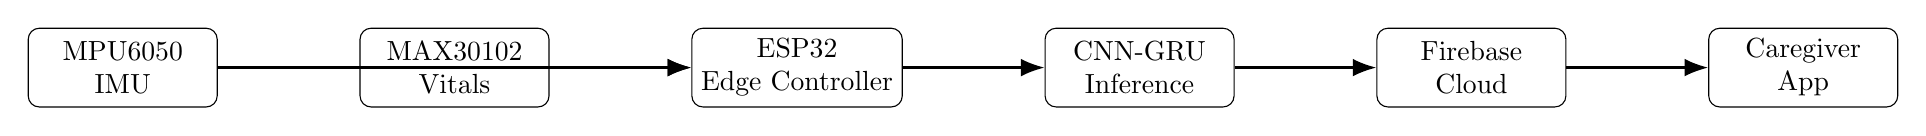
\begin{tikzpicture}[
node distance=1.8cm,
block/.style={draw, rounded corners, minimum width=2.4cm, minimum height=1cm, align=center},
arrow/.style={-{Latex[length=3mm]}, thick}
]
\node[block] (s1) {MPU6050\\IMU};
\node[block, right=of s1] (s2) {MAX30102\\Vitals};
\node[block, right=of s2] (s3) {ESP32\\Edge Controller};
\node[block, right=of s3] (s4) {CNN-GRU\\Inference};
\node[block, right=of s4] (s5) {Firebase\\Cloud};
\node[block, right=of s5] (s6) {Caregiver\\App};

\draw[arrow] (s1) -- (s3);
\draw[arrow] (s2) -- (s3);
\draw[arrow] (s3) -- (s4);
\draw[arrow] (s4) -- (s5);
\draw[arrow] (s5) -- (s6);
\end{tikzpicture}
\caption{Overall Guardian 360 system architecture.}
\label{fig:overall}
\end{figure*}

\section{Methodology}
Guardian 360 acquires inertial and physiological signals continuously using wearable sensors. Motion sequences are segmented using sliding windows and preprocessed through filtering, normalization, and sensor fusion. The resulting time-series windows are passed to a CNN-GRU classifier for motion understanding and risk estimation.

\subsection{Real-Time Fall Detection}
The MPU6050 captures tri-axial acceleration and angular velocity. Sudden impact magnitude, posture change, and motion discontinuity are analyzed for fall detection. Rule-based impact logic complements AI inference for fast fail-safe detection.

\subsection{Gait Analysis}
Walking sequences are analyzed to extract stride variability, motion asymmetry, instability, and abnormal locomotion signatures. These patterns form the basis for predictive fall risk estimation.

\subsection{Fall Risk Prediction}
Instead of detecting only completed falls, Guardian 360 identifies unstable gait progression and outputs a risk score prior to impact.

\section{CNN-GRU Model Architecture}
\begin{figure}[!t]
\centering
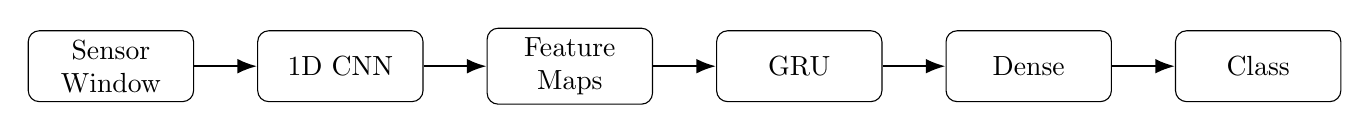
\begin{tikzpicture}[
node distance=0.8cm,
block/.style={draw, rounded corners, minimum width=2.1cm, minimum height=0.9cm, align=center},
arrow/.style={-{Latex[length=2.5mm]}, thick}
]
\node[block] (a) {Sensor\\Window};
\node[block, right=of a] (b) {1D CNN};
\node[block, right=of b] (c) {Feature\\Maps};
\node[block, right=of c] (d) {GRU};
\node[block, right=of d] (e) {Dense};
\node[block, right=of e] (f) {Class};
\draw[arrow] (a)--(b);
\draw[arrow] (b)--(c);
\draw[arrow] (c)--(d);
\draw[arrow] (d)--(e);
\draw[arrow] (e)--(f);
\end{tikzpicture}
\caption{CNN-GRU inference workflow.}
\label{fig:cnngru}
\end{figure}

The CNN-GRU architecture combines spatial feature extraction with temporal sequence modeling:

\subsection{CNN Layer}
The CNN extracts local motion signatures from short inertial windows, capturing abrupt acceleration changes, gait micro-patterns, and motion transitions.

\subsection{GRU Layer}
The GRU models temporal dependencies across motion sequences and learns instability progression over time.

\subsection{Dense Layer}
The output layer classifies:
\begin{itemize}[leftmargin=*]
\item Normal gait
\item Abnormal gait
\item Fall risk
\item Fall event
\end{itemize}

GRU is preferred over LSTM due to fewer parameters, lower memory consumption, reduced latency, and better embedded suitability.

\section{Dataset and Data Collection}
The model is trained using a combination of public and controlled datasets:
\begin{itemize}[leftmargin=*]
\item SisFall
\item MobiAct
\item UP-Fall Detection Dataset
\item Controlled unstable gait recordings
\item Simulated elderly fall sequences
\end{itemize}

Sensor streams include:
\begin{itemize}[leftmargin=*]
\item Tri-axial acceleration
\item Tri-axial gyroscope
\item Gait sequence windows
\item Impact transitions
\end{itemize}

Signals are sampled at \SI{50}{Hz}--\SI{100}{Hz}, segmented using sliding windows (2--4 s), normalized, and fused into multichannel inertial tensors.

\section{Hardware and Software Requirements}
\subsection{Hardware}
\begin{itemize}[leftmargin=*]
\item \textbf{ESP32:} low-power dual-core MCU with Wi-Fi/BLE and edge inference support
\item \textbf{MPU6050:} 6-axis IMU for motion and gait sensing
\item \textbf{MAX30102:} heart rate and SpO$_2$ monitoring
\item \textbf{GPS Module:} location tracking during emergencies
\item \textbf{OLED Display:} status and alert visualization
\item \textbf{Buzzer:} local emergency feedback
\item \textbf{SOS Button:} manual emergency trigger
\item \textbf{Rechargeable Battery:} portable low-power operation
\end{itemize}

\subsection{Software}
\begin{itemize}[leftmargin=*]
\item Arduino IDE
\item Embedded C
\item Python
\item TensorFlow / TensorFlow Lite
\item Firebase
\item TinyML deployment pipeline
\end{itemize}

\section{Experimental Setup}
Training is performed offline in Python using TensorFlow. Sensor windows are processed into multichannel inertial tensors and split into training, validation, and test sets. The trained model is quantized using TensorFlow Lite for ESP32 deployment.

\textit{Placeholder: Insert final train/validation/test split, optimizer, epochs, batch size, and quantized model footprint from implementation.}

\section{Results and Discussion}
Literature-guided analysis and architecture benchmarking suggest that CNN-GRU offers a strong balance between predictive performance and embedded efficiency. The model is expected to achieve high classification performance with low inference latency and improved pre-fall instability recognition.

\textit{Placeholder: Replace with measured implementation results before submission.}

Expected observations:
\begin{itemize}[leftmargin=*]
\item CNN-GRU improves temporal gait understanding over CNN-only models.
\item CNN-GRU provides lower latency and memory usage than CNN-LSTM.
\item Random Forest and SVM underperform on sequential instability progression.
\item Vision Transformers require higher compute and power, limiting wearable suitability.
\end{itemize}

\section{Comparative Analysis}
\begin{table*}[!t]
\centering
\caption{Analytical Comparison of Fall Analysis Models}
\label{tab:comparison}
\scriptsize
\begin{tabular}{lcccccc}
\toprule
Model & Accuracy & F1-score & Inference Speed & Memory Usage & Embedded Suitability & Fall Prediction \\
\midrule
SVM & Medium & Medium & High & Low & High & Low \\
Random Forest & Medium & Medium & Medium & Medium & Medium & Low \\
CNN-LSTM & High & High & Medium & High & Medium & Medium \\
Vision Transformer & High & High & Low & Very High & Low & High \\
\textbf{CNN-GRU} & \textbf{High} & \textbf{High} & \textbf{High} & \textbf{Medium} & \textbf{High} & \textbf{High} \\
\bottomrule
\end{tabular}
\end{table*}

\section{Advantages}
\begin{itemize}[leftmargin=*]
\item Predictive rather than reactive fall monitoring
\item Lightweight deep learning for edge deployment
\item Multimodal wearable sensing
\item Low-latency real-time inference
\item Caregiver connectivity and remote supervision
\end{itemize}

\section{Limitations}
\begin{itemize}[leftmargin=*]
\item Requires real-world elderly validation
\item Performance may vary across gait impairments
\item Battery life depends on sensing frequency and wireless usage
\item Limited contextual awareness beyond wearable motion
\end{itemize}

\section{Future Scope}
Future extensions include Tiny Transformers for efficient sequence learning, vision-assisted posture analysis, multimodal emotion and cognitive monitoring, smart home integration, federated learning, and further edge optimization for continuous adaptive elderly care.

\section{Conclusion}
Guardian 360 presents a practical and lightweight embedded AI framework for elderly safety monitoring using wearable sensing and CNN-GRU-based predictive analytics. By combining gait analysis, fall risk prediction, physiological monitoring, and emergency communication in a single wearable platform, the proposed system advances elderly care from reactive monitoring to proactive intervention. The proposed architecture is computationally efficient, implementation-oriented, and suitable for low-power real-time deployment, making it a promising solution for next-generation predictive elderly healthcare systems.

\balance
\bibliographystyle{IEEEtran}
\begin{thebibliography}{99}

\bibitem{salma2025}
I.~Salma \textit{et al.}, ``Remote monitoring system for older adults at risk for complications: a scoping review,'' \textit{BMC Geriatrics}, 2025.

\bibitem{bandara2020}
A.~Bandara \textit{et al.}, ``A sensor platform for non-invasive remote monitoring of older adults in real time,'' 2020.

\bibitem{setu2025}
S.~S.~Setu \textit{et al.}, ``A novel approach for a smart IoMT-based BAN for old home healthcare monitoring system,'' \textit{arXiv}, 2025.

\bibitem{setu2024}
S.~S.~Setu \textit{et al.}, ``Smart home solutions for elderly care,'' 2024.

\bibitem{augastiny2023}
R.~Augastiny \textit{et al.}, ``IoT based health monitoring system for aged people using NodeMCU,'' 2023.

\bibitem{saraubon2018}
K.~Saraubon \textit{et al.}, ``A smart system for elderly care using IoT and mobile technologies,'' in \textit{Proc. ACM}, 2018.

\bibitem{gaud2025}
N.~Gaud \textit{et al.}, ``FIBiLS: Fall detection of healthy elderly using IMU sensor and BiLSTM model,'' \textit{IEEE Sensors Journal}, 2025.

\bibitem{li2024}
Y.~Li \textit{et al.}, ``Deep learning framework for fall detection,'' \textit{Cognitive Computation}, 2024.

\bibitem{zhang2025}
Zhang \textit{et al.}, ``AI for fall detection in older adults,'' 2025.

\bibitem{lim2024}
Z.~K.~Lim \textit{et al.}, ``Fall risk prediction using temporal gait features and machine learning approaches,'' \textit{Frontiers in AI}, 2024.

\bibitem{tsiakiri2025}
A.~Tsiakiri \textit{et al.}, ``Wearable sensor technologies and gait analysis for early detection of dementia,'' \textit{Sensors}, 2025.

\bibitem{ishaq2026}
M.~Ishaq \textit{et al.}, ``A systematic review of fall detection and prediction technologies for older adults,'' \textit{Applied Sciences}, 2026.

\bibitem{patel2023}
Patel \textit{et al.}, ``Wearable sensor-based fall detection review,'' 2023.

\bibitem{alkhafajiy2019}
M.~Al-khafajiy \textit{et al.}, ``Remote health monitoring of elderly through wearable sensors,'' \textit{Multimedia Tools and Applications}, 2019.

\bibitem{deshmukh2026}
S.~Deshmukh, ``An IoT-enabled smart healthcare monitoring system using machine learning for early health risk prediction,'' 2026.

\bibitem{rahmani2024}
M.~H.~Rahmani \textit{et al.}, ``EmoWear: wearable physiological and motion dataset for emotion recognition,'' \textit{Scientific Data}, 2024.

\bibitem{huang2024}
L.~Huang \textit{et al.}, ``Automatic speech analysis for detecting cognitive decline of older adults,'' \textit{Frontiers in Public Health}, 2024.

\bibitem{attal2015}
F.~Attal \textit{et al.}, ``Physical human activity recognition using wearable sensors,'' \textit{Sensors}, 2015.

\bibitem{wang2024}
Wang \textit{et al.}, ``WiFi CSI-based fall detection,'' 2024.

\bibitem{carefall2023}
``CareFall: AI-based wearable system,'' \textit{arXiv}, 2023.

\end{thebibliography}

\end{document}